The algorithm proposed by Harms is well designed but is not capable of finding similar user sequences. 
When there is more than one possible interaction to achieve a goal, the method of Harms will create two different sequences for that interaction, 
or worse, will not detect the interaction as a meaningful one at all. For this reason I propose an algorithm that is able to detect similar subsequences.
The basic steps of the algorithm do not differ alot from Harms one. In fact some preprocessing steps and the sequence detection have been altered.
Algorithm \ref{alg:tasktreeoverview} shows the main building blocks and will function as a list and order of contents of this chapter.
\section{Task Tree Generation}

\begin{algorithm}[h]
\floatname{algorithm}{Algorithm}
\begin{algorithmic}
	\Procedure{GenerateTaskTree}{UserSessions}
	\State Generate Substitution Matrix (UniqueTasks)
	\While{Replaced Tasks} 
	\State Detect Iterations (UserSessions)
	\State Optional: Substitution Matrix Update
	\State Detect Sequences (UserSessions,SubstitutionMatrix)
	\EndWhile
	\EndProcedure
\end{algorithmic}
\caption{Overview over the task tree generation}
\label{alg:tasktreeoverview}
\end{algorithm}

\section{Task Distance Substitution Matrix}
The harmonization process performed by Harms et al. is also applied to the user sessios in this approach. 
A useful side product of the harmonization is the set of unique tasks.
This set is needed for this step of the algorithm, the generation of the substitution matrix.

In section \ref{sec:foundationsubstitutionmatrix} we introduced substitution matrixes in general and what they are good for. 
For this use case we needed to generate one substitution matrix that represents how similar tasks are. 
The score of two tasks in the \textit{task distance substitution matrix} is defined as follows:
\begin{definition}
	\item Let a and b be two tasks
	\item Let S(a,b) be the score for substituting task a with task b. The higher the value of S is, the more similar are the tasks a and b and vice versa.
\end{definition}

To calculate the score, three cases have to be considered:
\begin{itemize}
	\item Similarity of two event-tasks
	\item Similarity of an event-task and a non-event-task
	\item Similarity of two non-event-tasks
\end{itemize}

\subsection{Event-Task Event-Task Similarity}
The first idea was to calculate the score of the matrix based on the distance between the absolute coordinates of the events-tasks. 
There are a few problems with this approach: First, not all event-tasks may have absolute coordinates. 
The second problem with this method is that in graphical user interfaces events may still be very similar, even if they have a large absolute distance.
An example for such a case would be a web formular with many fields to fill out. 
TODO: Maybe Screenshot here?
Those fields take space which would result in large distances between them although the event-tasks all belong to a single formular.
The solution to this problems is to make use of a grouping of elements the designer of the GUI already did: The GUI-Model (see section \ref{sec:foundationguiandguimodel}).
Elements of a GUI that belong to one semantic task can usually be found in some kind of container that groups those elements together. Therefore the basis for my 
distance calculation is the distance in the GUI-Model, as defined in \ref{def:guimodeldistanceee}. 

\begin{definition}
	\item Let a and b be events-tasks
\begin{equation*}d(a,b) = d(b,a) = \text{the distance in the GUI model of the targets of event-tasks a and b.}
\end{equation*}
\label{def:guimodeldistanceee}
\end{definition}

Since the GUI model is a tree, the distance of two targets in a GUI can easily be calculated by finding the common ancestor of the targets and summing up the number of nodes from both the events to this ancestor, including the ancestor.
\begin{figure}
\begin{center}
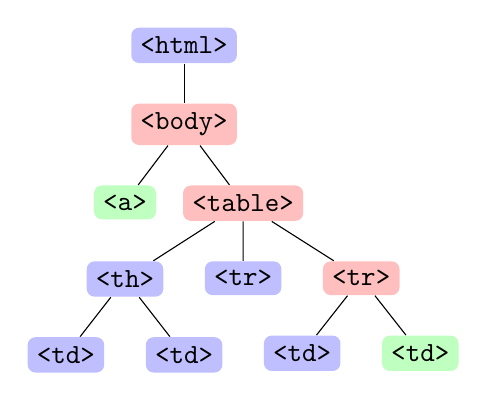
\begin{tikzpicture}[
    fact/.style={rectangle, draw=none, rounded corners=1mm,
        text centered, anchor=north, text=black, fill=blue!25},
    redcolor/.style={rectangle, draw=none, rounded corners=1mm,
        text centered, anchor=north, text=black, fill=red!25},
    greencolor/.style={rectangle, draw=none, rounded corners=1mm,
        text centered, anchor=north, text=black, fill=green!25},
    level distance=0.5cm, growth parent anchor=south]

\node (Fact01) [fact] {\texttt{<html>}} [-]
    child{
        node (kolor4) [redcolor] {\texttt{<body>}}
        child{
            node (color1) [greencolor] {\texttt{<a>}}
        }
        child{
            node (Fact04) [redcolor] {\texttt{<table>}}
            child{
                node (Fact05) [fact] {\texttt{<th>}}
                child{
                    node (fact5) [fact] {\texttt{<td>}}
                }
                child{
                    node (Fact07) [fact] {\texttt{<td>}}
                }
            }
	    child{
                node (Fact05) [fact] {\texttt{<tr>}}
	    }	
            child{
                node (color3) [redcolor] {\texttt{<tr>}}
                child{
                    node (Fact10) [fact] {\texttt{<td>}}
                }
                child{
                    node (color2) [greencolor] {\texttt{<td>}}
                }
            }
        }
    }   
;
 
\end{tikzpicture}
\end{center}	
\label{fig:guimodeldistance}
\caption{A HTML GUI model with two nodes (green) the distance will be calculated for.  The number of red nodes is the distance between the green nodes. The common anchestor is the \texttt{<body>} element.}

\end{figure}
Figure \ref{fig:guimodeldistance} shows a GUI model with two elements and their common ancestor. 


\subsection{Event-Task Non-Event-Task Similarity}
It takes a bit more effort to calculate the substitution score if one task is a non-event-task. 
The reason is that the non-event tasks do not represent a simple event anymore. Therefore they do not possess a target in the GUI.
A possible solution is to recursively visit every child of the non-event-task, gather all event tasks and then calculate the mean distance from each of those tasks to the event-task the distance shall be calculated to.
Formally, definition \ref{def:guimodeldistanceee} has to be modified so that it covers non-events as well:

\begin{definition}
%	\item Let a and b be events-tasks, then:
%\begin{equation*}d(a,b) = d(b,a) = \text{be the distance in the GUI model of the targets of event-tasks a and b.}
%\end{equation*}
	\item Let c be a non-event-task
	\item Let E be the set containing all event-tasks that can be recursively found in c.
	\item with definition \ref{def:guimodeldistanceee} it is possible to define d as
\begin{equation*}
	d(a,c) = d(c,a) = \frac{\sum_{\forall x \in E} d(a,x)}{|E|}
\end{equation*}
\label{def:guimodeldistanceene}
\end{definition}

\subsection{Non-Event Non-Event Similarity}
With Definition \ref{def:guimodeldistanceene} it is simple to compute the distance for two tasks since all that is to do now is to repeat the procedure of finding all event-task children of one task, calculate the distances to the other task and use the mean distances as the total distance.
The definition of d can be extended so it accepts two non-event-tasks:

\begin{definition}
	\item Let c and d be non-event-tasks 
	\item Let E be the set containing all event-tasks that can be recursively found in c.
	%\item Let F be the set containing all event-tasks that can be recursively found in d.
	\item with definition \ref{def:guimodeldistanceene} it is possible to define d as
	\begin{equation*}
		d(c,d) = d(d,c) = \frac{\sum_{\forall x \in E} d(x,d)}{|E|}
	\end{equation*}
\label{def:guimodeldistancenene}
\end{definition}
\subsection{Score}
Now that I defined the distance for three cases it is possible to compute the score $S$ of two tasks.
\begin{definition}
	\item Let U be the set of unique tasks occurring in the user sessions
	\item Let k be a constant that defines the maximal score 
	\item For each tupel $i,j \in U$ 
\begin{equation*}
		 S(i,j) = -1*d(i,j)+k
	\label{eq:subscore}
\end{equation*}
\end{definition}

The k constant should be chosen dependent on the underlying GUI model. A large k should be chosen for very deeply, nested GUI models whereas for flat GUI models a smaller k seems better. 

The maximal score is reached if the distance between two elements is zero. This happens if we compare two equal elements.
A problem can occur when the score of a non-event-task to an event task is equal to maximal score. 
This happens if a non-event-task has just one event-task as child and the distance of this child to the same event-task is calculated. 
Since it is preferred that the score of two equal event-tasks is always larger than the score of this event-task with a non-event-task we add the penalty term $L$ to the score equation.

\begin{definition}
	\item Let E be the set of all event-tasks
	\item let N be the set of all non-event-tasks
\begin{eqnarray*}
	L(i,j) &=& 
	\begin{cases}
		0 & \text{if } i,j \in E \\
		\text{constant} & \text{if } i \in N \lor  j \in N\\
	\end{cases} \\
	S(i,j) &=& -1*d(i,j)+k-L
\end{eqnarray*}
	\label{eq:subscore_adjusted}
\end{definition}


\section{Iteration Detection and Substitution Matrix Update}
The iteration detection from Harms is also suitable for my algorithm was not altered in any way. It reliably detects iterations and replaces them in the user sessions.
Before the sequence detection can come to play the substitution matrix should be updated since there were new iteration tasks created during iteration detection. Those new tasks are stored in a set that contains all newly created tasks.
The update process differs just a little from the generation process with the only difference beeing that just the distances between the newly created tasks to the current set of unique tasks is as well as the distances between the newly created tasks are computed.
After the matrix has been updated, the newly created tasks are merged with the set of unique tasks and then emptied.
TODO: NOT UP TO DATE The whole step of updating the matrix is currently implemented but not used. 
Instead, each score between an event-task to a non-event-task and therefore all scores between non-event-tasks are defined as zero due to perfomance issues.
More details on this issue can be found in section TODO: REF HERE.

\section{Sequence Detection}
As we figured out at the beginning of this chapter the sequence detection is the part of the algorithm that varies the most from Harms approach.
It is itself separated in three steps:
\begin{itemize}
	\item The search for significant patterns
	\item The model generation
	\item The sequence replacement
\end{itemize}

\subsection{Search for significant patterns}		
The search for significant patterns is done with an alignment method we introduced in section \ref{sec:alignments}. 
The bioinformatical problem of comparing and aligning DNA/RNA/Amino acid sequences is closely related to finding important subsequences in the user sessions. 
The conserved regions of biological sequences comply with those interactions that most of the users performed similarly. 
We can conclude that those interactions are meaningful in the sense of fulfilling one desired task.
The goal of the alignment algorithm is now to detect the conserved regions and extract a model of the average user behaviour. 
Since alignment algorithms also find approximate and not only exact similarities, this step of the sequence detection is the main difference to Harms method.

The first step of the search for significant patterns is to align every user session with any other user session with an algorithm called Smith-Waterman algorithm for repeated matches.
For the rest of this section the user session will be represented by a sequence of numbers. Each number in a sequence corresponds with the unique id the task at this position in the user sessions has.
We now describe the algignment algorithm in detail.

\paragraph{Smith Waterman Algorithm For Repeated Matches}
The Smith-Waterman algorithm for repeated matches\cite{durbin1998} is a modified version of the original Smith-Waterman algorithm\cite{waterman1981}.
The original Smith-Waterman finds the best local similarity between two sequences.
Since we need all relevant similarities and not just the one with the best score, we define a threshold score $T$.
Once a local subalignment reaches T it is considered as relevant.

We recall from the alignments introduction that alignment algorithms try to find the best possible score between two sequences using the underlying scoring model of substitution and gap scores.
The most na\"ive approach is to try out all possible combinations both sequences could be aligned. As usual, this approach is not very feasible because there are 
\begin{equation*}
	\binom{2n}{n} = \frac{(2n)!}{(n!)^2} \simeq \frac{2^{2n}}{\sqrt{\pi n}}
\end{equation*}
possible global alignments of two sequences\cite{durbin1998}. 
Another way would be to use some kind of heuristic but we are interested in an exact, deterministic method.
A common technique to solve this issue is dynamic programming\cite{bellman1957}. 
The main idea of dynamic programming is not to calculate every possible variant but to reuse the best solutions of smaller subproblems.  
This method is central to computational sequence analysis\cite{durbin1998}.

\subparagraph{Basic Smith-Waterman}
The basic version of the Smith-Waterman algorithm makes use of dynamic programming by defining the dynamic programming matrix $F$ where each cell of the matrix stores the best score for aligning the elements up to the position the cell represents.
For example the cell $(2|2)$ stores the score for the best alignment of first two elements of each sequence. 
Each cell is computed by getting the best score out of four choices. Prior to enlisting those, we need the following definitions: 

\begin{definition}
	\item Let x,y be two sequences
	\item Let F be a matrix with F(i,j) being the best score of aligning $x_1\dots x_i$ with $y_1\dots y_j$
\end{definition}

Then we can compute F by repeatedly applying the following equation:
\begin{equation}
F(i,j) = max \left\{ \begin{array}{lr}0,&\\F(i-1,j-1)+S(x_i,y_j),&Substitution\\F(i-1,j)-g,&Gap\\F(i,j-1)-g.&Gap\\\end{array} \right. 
\end{equation}
Figure \ref{fig:basicalignmentoperations} illustrates this formula. The diagonal choice means we align one element from each sequence with each other. Therefore we have to look up the similarity of both elements in the substitution matrix. 
When the score from the upper cell minus the gap penalty is bigger than the diagonal choice a gap will appear at this position in sequence y. 
This is the same for when the option from the left cell is taken, just that the gap will be inserted in sequence x. 
The option 0 in the equation is to prevent alignment scores to become negative. 
If a match cannot be extended with its score being a positive value it is better to start a new one later. 
As we can see it is possible to fill the whole matrix by once the trivial scores, the first row and the first column, have been initialized.

\begin{figure}
	\centering
	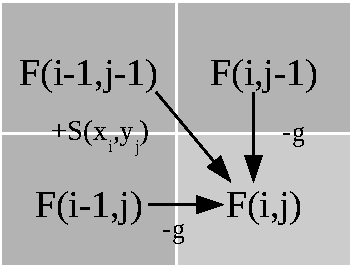
\includegraphics{img/basic_cell_fill.pdf}
	\caption{Illustration of the three operations deletion, insertion and substitution in a dynamic programming matrix}
	\label{fig:basicalignmentoperations}
\end{figure}

\subparagraph{Repeated matches}
In the improved version of the algorithm a cell in F has a slight different meaning and its computation is a bit more complex. 
The first difference is that this algorithm is asymetric in the sense of aligning sequence x to sequence y produces a different outcome than aligning sequence y to sequence x. Hence, we define y as the pattern we want to search and x as the sequence in which we search all subsequences of y repeatedly.
This results in a final alignment where x has matched and unmatched regions.  

The algorithm itself is partitioned into three parts: 

\begin{itemize}
	\item Initialization
	\item Recursion
	\item Traceback
\end{itemize}

\subparagraph{Intialization:}
	The initialization step is simple: \\
	Let m be the length of y
	
	\begin{equation*}
		F(0,j) = 0 \text{ for } j=0\dotsc m
	\end{equation*}
	This differs from the Smith-Waterman algorithm described by Durbin et al.\cite{durbin1998} who just initialize F(0,0) and do not fill the first column. There is no need to initialize the first row because a subalignment will never start with a gap. For the sake of an easy implementation it was better to initialize the first row though.

\subparagraph{Recursion}
The recursion formula for filling the matrix also has the three options for insertion/deletion and substitution as illustrated in figure \ref{fig:basicalignmentoperations}.
But as we see there are some more options. 
For the first row (equation \ref{eq:firstrow}), which does not represent a real alignment of sequences but denotes the sum of completed match scores, we have two options. 
The first one is to take the the the value from the last column so we always keep track of the total score. 
This leads to the fact that the value in this line will always stay the same or increase, but never decrease.
The second choice is taken when a match reaches its maximum and has a minimum score of T. 
This is the consequence of an ending match meaning this choice is just taken when we calculate the cell for an unmatched region.
To summarize the equation for the first row we can say the algorithm choses the maximum value of the last column minus T or adopts the value of the preceding cell in the first row, depending which one was larger. 

Equation \ref{eq:otherrows} for the fields aside of the first row is amended by the posibility to begin its alignment score with the value standing in the first row of its own column. 
Durbin et al. does not mention the fact that this makes it easier for subalignments of long sequences to reach the threshold score once a few matches have been found before.
This issue has not been investigated in this work. 
The total score of the whole alignment is stored in F(i+1,0). This cell lies an unmatched region of x and contains the sum of all completed match scores.


\begin{equation}
F(i,0) = max \left\{ \begin{array}{lr}F(i-1,0),&\\F(i-1,j)-T,& j=1,\dots,m\end{array}\right. 
\label{eq:firstrow}
\end{equation}
\begin{equation}
F(i,j) = max \left\{ \begin{array}{lr}F(i,0),\\F(i-1,j-1)+S(x_i,y_i),\\F(i-1,j)-g,\\F(i,j-1)-g.\end{array}\right.
\label{eq:otherrows}
\end{equation}
		
\subparagraph{Traceback}
A very important point in dynamic programming algorithms is that we not just calculate and store the maximum score for each subalignment but additionally have to store which choice of the formula produced the highest value.
This makes it possible to go back from the total best score to the start and find the actual alignment of the whole sequences. This process is called traceback. 
Figure \ref{fig:durbindpmatrixtraceback} shows a completly filled dynamic programmic matrix and the traceback path.

\begin{figure}
\centering
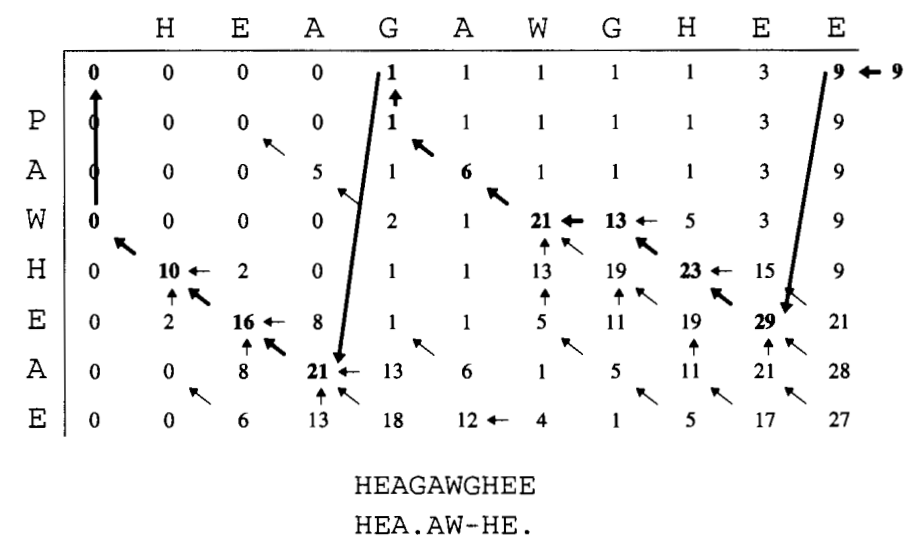
\includegraphics[scale=0.4]{chapters/approach/smithwatermanrepeated.png}
\caption{Figure from Durbin et al.\cite{durbin1998}. The repeat dynamic programming matrix for two example sequences, for T = 20. Below the optimal alignment, with total score $9 = 29-20$. There are two separate match regions, with scores 1 and 8. Dots are used to indoicate unmatched regions of x. The arrows show the traceback process, going back from the total score to the start.}
\label{fig:durbindpmatrixtraceback}
\end{figure}

\subparagraph{Match retrival}
To find similar user behaviour we are just interested in the matches that reached the threshold score. After aligning every user session with each other we extract all matches from those alignments.
We consider every subset of the alignment that is not a unmatched region a match.
Therefore a match consists of two sequences of numbers and can contain gaps. We will encode a gap in the number -1. 
Fig \ref{fig:matchexample} shows an example of a match, containing one gap in the first sequence, two exact tasks and one substitution.


\begin{figure}[h]
	\centering
	\begin{tabular}{cccc}
		9 & 16 & -1 & 6 \\
		9 & 15 & 17 & 6  
	\end{tabular}
	\caption{Example for a retrieved match}
	\label{fig:matchexample}
\end{figure}
	\begin{itemize}
		\item Search match in all user sessions
		\item From the most to the least found match:
	\end{itemize}
\subsubsection{Model generation}
	\begin{itemize}
		\item Generate Model From Match is done the following way:
		\item For each position of the Match: 
		\item (remind, that each match has 2 Sequences of aligned numbers)
		\begin{itemize}
			\item If Both numbers are equal: The model at this position is the Task refered by this number
			\item If one sequence has a gap at this position: The other EventTask is inserted as an optional
			\item If both numbers differ a selection is inserted. Which kind of selection depends on what the following task is. We don't want to have 2 selections next to each other, instead, create one selection and add each sequence as a sequence
			\begin{itemize}
				\item If the next position also would be a selection, the selection has 2 sequences as a child. those sequences consists of the tasks of each sequence of the match until there is no more selection found 
				\item If the next position is something else we just have a single selection, just add the tasks of the match at this position as childs to the selection
				\item (This description here is really bad, will need some examples)
			\end{itemize}
		\end{itemize}
	\end{itemize}

\subsubsection{Replacement}
	\begin{itemize}
		\item Replace each model in the user sessions
	\end{itemize}

\subsection{Repetition}



